% !TEX root=ricardo_draft.tex
%%% TeX-master: "ricardo_draft"~\ref{figure.simple_models}
\begin{figure*}[th!]
\begin{center}
\vspace{-2ex}
\centerline{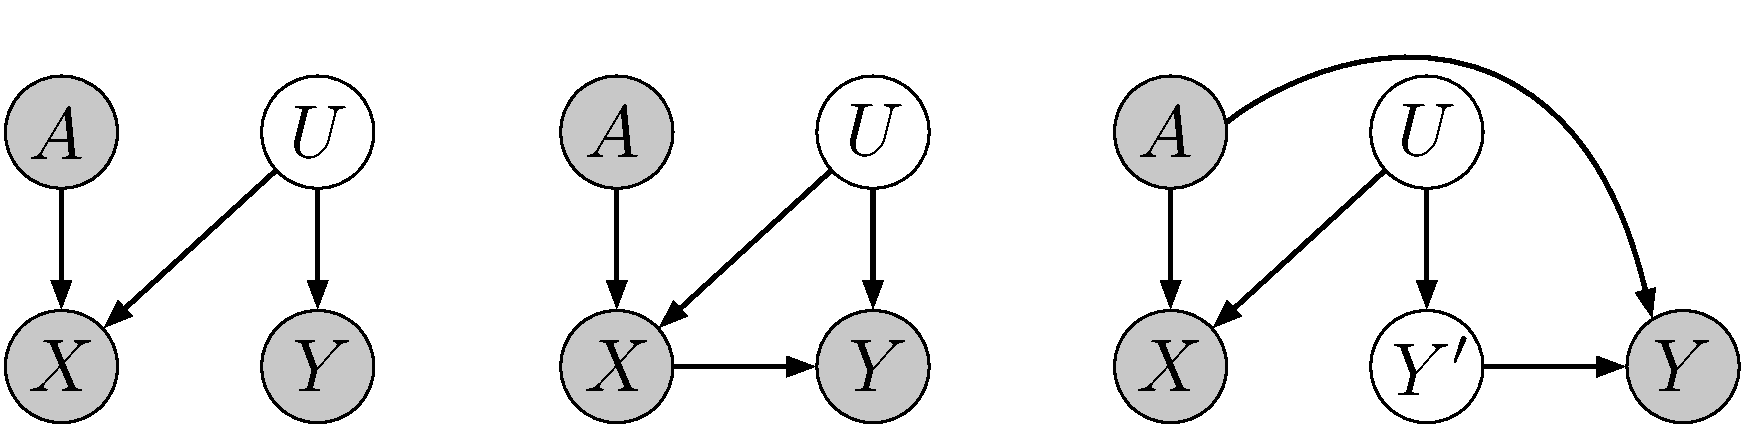
\includegraphics[width=\textwidth]{simple_models_no_q}}
\vspace{-2ex}
\caption{Three possible states of the world.\label{figure.simple_models} See section \ref{sec:count_fair} for discussion.}
\vspace{-2ex}
\end{center}
\end{figure*}

When describing counterfactual fairness, it is important to
distinguish between a counterfactually fair {\em world} in which the
variable $Y$ we are interested in predicting is inherently
counterfactually fair with respect to the protected attributes $A$,
and a counterfactually fair {\em predictor} $\hat Y$, guaranteed to
be counterfactually fair, regardless of the behavior of $Y$.

Figure~\ref{figure.simple_models} shows possible worlds. {\em Left:} A
counterfactually fair world in which the state of $Y$ has no
dependencies on $A$. {\em Center and Right:} Potentially unfair worlds
in which the state of $A$ can influence the state of $Y$ either
indirectly as in {\em center} or directly as in {\em Right}.

To provide intuition, we outline simple scenarios corresponding to each world:
\paragraph{Left: The Red Car.}
Imagine a car insurance company wishes to price insurance for car owners by
predicting their accident rate $Y$. We assume there is $U$, an
unobserved factor corresponding to aggressive driving, that causes
drivers to be more likely have an accident, and that aggressive
individuals are more likely to prefer to drive red cars (our observed
variable $X$). Moreover, we assume that individuals belonging to a
protected attribute ($A$) are more likely to drive red cars, but
importantly, they are no more likely to be aggressive or to get in
accidents than any one else.


\paragraph{Center: High Crime regions} We're interested in predicting
the likelihood of a particular individuals house being broken in to
$Y$. This likelihood may depend on a variety of unobserved factors
($U$) but also upon the neighborhood the house lies in ($X$), and the
neighborhood an individual lives in may be strongly correlated with
race $A$. In such a scenario, although the likelihood of a particular
person having their house broken into does not depend upon race
directly, it does vary which a persons race and so is not
counterfactually fair.

\paragraph{Right: Prejudicial Estimation} The world on the right shows $Y'$ a
causally fair variable that doesn't depend on $A$ being directly
corrupted by a bias relating to $A$, resulting in an observation
$Y$. In this case, learning a causally fair approximation of $Y$ can
recover the true variable $Y'$ (up to noise).
Rdef
\subsection{Definition}
Formally, a variable $Y$ is said to be counterfactually fair with
respect to a protected attribute $A$ if
\begin{define}[Counterfactually Fair] setting variable $A$ to a
  particular state as detailed by \ref{subsec:cmc} does not alter the
  probability of $Y$ taking a particular state.
\begin{equation}
P(Y)=P(Y=y|\text{do}(A=a))\forall a,y 
\end{equation}
\end{define}
This definition substantially differs from Fairness Through
Unawareness, as it considers the influence of attributes such as race
on other measured variables.

% TODO. Here the main
% definition is introduced, and how it relates to ``path deletion'',
% including the core example of $A \rightarrow X \rightarrow Y$, with
% two latent variables $U_x \rightarrow X$ and $U_y \rightarrow Y$,
% arguing that one might judge that the path from $A$ to $Y$ via is due
% to an unfair mechanism and that we need a notion of ``closest world''.

\subsection{Examples}
To get an intution for what the different definitions of fairness imply, we will
revisit the examples of figure \ref{figure.simple_models}.
% begin by describing a few possible real-world scenarios. For each of these we will describe what counterfactually-fair and counterfactually-unfair predictors look like.

\paragraph{Scenario 1: The Red Car.}
Imagine a car insurance company wants a quick, anonymous way to determine how to price insurance for different car owners by predicting their accident likelihood $Y$. They've noticed that there is a correlation between driving a red car $X$ and a higher rate of automobile accidents. Thus they would like to increase the insurance for all red car drivers. 

Imagine what's really going on is shown in Figure~\ref{figure.simple_models} (\emph{Left}). The correlation between have a red car $X$ and accidents $Y$ is due to an `aggressiveness' factor $U$: aggressiveness causes individuals to be in accidents more often, and it also attracts them to red cars. Unfortunately, the red car feature $X$ is also affected by an individual's race $A$. 

Thus, simply using $X$ to predict $Y$ would seem to be an unfair prediction because it may charge individual's of a certain race more than others. Counterfactual fairness agrees with this. 

\begin{lem}
The predictor $\hat{Y}(X)$ is not counterfactually fair for the model in Figure~\ref{figure.simple_models} (\emph{Left}).
\end{lem}

\begin{proof}
For simplicity, let's imagine that the equations described by the model in Figure~\ref{figure.simple_models} (\emph{Left}) are deterministic and linear:
\begin{align}
X = \alpha A + \beta U, \;\;\;\; Y = \gamma U \nonumber
\end{align}
where the coefficients $\alpha,\beta,\gamma$ are given (in practice we will estimate these). We can test whether a predictor $\hat{Y}(X)$ is counterfactually-fair using the procedure described in Section~\ref{subsec:cmc}:
\begin{itemize}
\item Compute $U$ given observations of $X,Y,A$, by solving for $U$.
\item Substitute the equations involving $A$ with an interventional value $a'$ (i.e., this says: `what happens if the race of an individual were changed')
\item Compute the variables $X,Y$ with the interventional value $a'$
\end{itemize}
In this deterministic case we achieve counterfactual fairness only if the predicted value $\hat{Y}(X)$ is identical before and after we change $A$. However, note that changing $A$ causes $X$ to change. Thus $\hat{Y}(X)$ must be different and so our model based on using $X$ to predict $Y$ is not counterfactually fair.
\end{proof}
Note that the above proof is without loss of generality: any model constructed using $X$ alone will not be counterfactually fair as changing $A$ will always have an influence on $X$.


TODO. Here the examples and their motivation can be as follows:

\begin{itemize}
\item something analogous to the red car example: $A$ is not a cause of
  $Y$ but might indirectly bias the result even without using $A$ as a predictor;
\item something with selection bias, maybe a toy version of COMPAS;
\item something where an unfair judgement (say, credit score) that can be potentially
  considered as a target variable, and an
  ``objective target'' (say, defaulting on a loan) are present, and
  what the recommendation is
\end{itemize}
%%% Local Variables:
%%% mode: latex
%%% TeX-master: "ricardo_draft"
%%% End:
